\documentclass[11pt,a4paper]{article}
\usepackage[margin=1in]{geometry}
\usepackage{amsmath,amssymb}
\usepackage{booktabs}
\usepackage{graphicx}
\usepackage[numbers]{natbib}
\usepackage{hyperref}
\usepackage{xcolor}
\usepackage{caption}

\captionsetup{font=small,labelfont=bf}
\graphicspath{{../figures/}}
\setlength{\bibsep}{2pt}
\renewcommand{\bibfont}{\small}

\title{Curation Orthogonality in Instruction-Tuning Data}

\author{Seil Kang \and Woojung Han \and Claw\thanks{Corresponding author} \and Claude Code\footnotemark[1]}
\date{}

\begin{document}
\maketitle

\begin{abstract}
We present a nonparametric statistical analysis of five quality dimensions---accuracy, relevance, conciseness, diversity, and information density---across two instruction-tuning corpora: Alpaca ($N = 51{,}974$) and WizardLM ($N = 51{,}923$).
Our strongest evidence comes from the two statistical dimensions with full score coverage (diversity and information density): they exhibit near-zero rank dependence (Kendall's $\tau = -0.025$) and produce top-30\% subsets with only 15.4\% overlap ($J = 0.154$, close to the random null $J_{\text{null}} = 0.176$).
Bootstrap validation on fully LLM-scored subsamples ($K = 5$, $N = 1{,}000$, no imputation) confirms that the accuracy--relevance pair shows moderate association ($\tau = 0.442 \pm 0.014$ in Alpaca), while cross-group pairs remain near-independent ($|\tau| < 0.08$).
Permutation tests (1{,}000 iterations) support 5 of 10 pairs as statistically detectable ($p < 0.01$, Benjamini--Hochberg corrected); the remaining pairs are consistent with independence.
The independence structure is dataset-dependent: WizardLM reveals elevated inter-correlation among statistical dimensions ($\tau$ up to $0.499$), suggesting that synthetic evolutionary generation introduces shared structural artifacts absent in human-curated data.
A downstream finetuning experiment on Qwen3.5 (0.6B and 2B)~\cite{qwen2025qwen3} confirms that score-level divergence translates to behavioral differences: diversity-optimized subsets produce models with $+5.2$pp higher Distinct-2 and $-6.9$pp lower Self-BLEU than universal filtering.
These results demonstrate that, for the quality operationalizations studied here, composite filtering sacrifices dimension-specific signal, though the magnitude varies with dataset provenance.
\end{abstract}

\section{Introduction}

The data-centric AI paradigm has established that training data composition matters as much as model architecture~\cite{hoffmann2022chinchilla}.
Zhou et al.~\cite{zhou2023lima} showed that 1{,}000 carefully curated examples can align a 65B-parameter model competitively, elevating data quality to a first-class concern.
Subsequent work---the Phi models~\cite{gunasekar2023phi}, DataComp-LM~\cite{gadre2024datacomp}---reinforced this through aggressive curation.
Yet a common pattern persists: ``quality'' is defined through a single composite filter, resting on the unstated assumption that high-quality data is high-quality along all dimensions simultaneously.

No prior work tests this assumption directly.
QuRating~\cite{wettig2024qurating} introduced multi-dimensional quality scoring for pretraining data but did not examine whether dimensions produce independent subsets.
HelpSteer2~\cite{wang2024helpsteer2} annotates five quality dimensions for reward-model training but does not test whether the induced subsets are independent.
QDIT~\cite{bukharin2024qdit} balances quality against diversity during instruction-tuning curation yet still reduces both to a single selection score.
DoReMi~\cite{xie2023doremi} optimizes domain-level mixtures but does not address within-domain quality dimensions.

We fill this gap with a simple experimental design: score each example in two instruction-tuning datasets across five quality dimensions, select top-30\% subsets per dimension, and measure rank correlation, set overlap, and quality loss from universal filtering.
Our analysis is entirely nonparametric---Kendall's $\tau$, Jaccard similarity, Mann--Whitney $U$, and permutation tests---avoiding distributional assumptions inappropriate for LLM-generated quality scores.

\section{Method}

\textbf{Data.}
We analyze Alpaca ($N = 51{,}974$; GPT-3.5-based self-instruct from human seeds) and WizardLM ($N = 51{,}923$; evolutionary synthetic generation, subsampled with seed~42).

\textbf{Quality dimensions.}
We define five dimensions spanning semantic and structural quality:
\emph{accuracy} ($q_{\text{acc}}$) and \emph{relevance} ($q_{\text{rel}}$) via LLM-as-judge (gpt-4.1-mini, $T=0$, 200-sample subsample, median imputation);
\emph{conciseness} ($q_{\text{conc}}$) via hedging-rate and length penalty;
\emph{diversity} ($q_{\text{div}}$) combining embedding distance from centroid (weight 0.6) with distinct-2 ratio (0.4);
\emph{information density} ($q_{\text{info}}$) combining compression ratio with word-level Shannon entropy (equal weights).

\textbf{Curation protocol.}
For each dimension $q_k$: (1) min-max normalize scores to $[0,1]$; (2) select the top-30\% subset $S_{q_k}$; (3) compute the universal baseline $q_{\text{univ}} = \frac{1}{5}\sum_k \tilde{q}_k$ and select its top-30\%.

\textbf{Statistical tests.}
Kendall's $\tau$ measures rank dependence between scoring vectors.
Jaccard index $J = |S_i \cap S_j| / |S_i \cup S_j|$ quantifies subset overlap (null expectation $J_{\text{null}} \approx 0.176$ for independent 30\% subsets).
Mann--Whitney $U$ with rank-biserial $r$ compares score distributions.
Permutation tests (1{,}000 iterations, 5{,}000-sample subsets) assess significance.

\section{Results}

\begin{figure}[t]
  \centering
  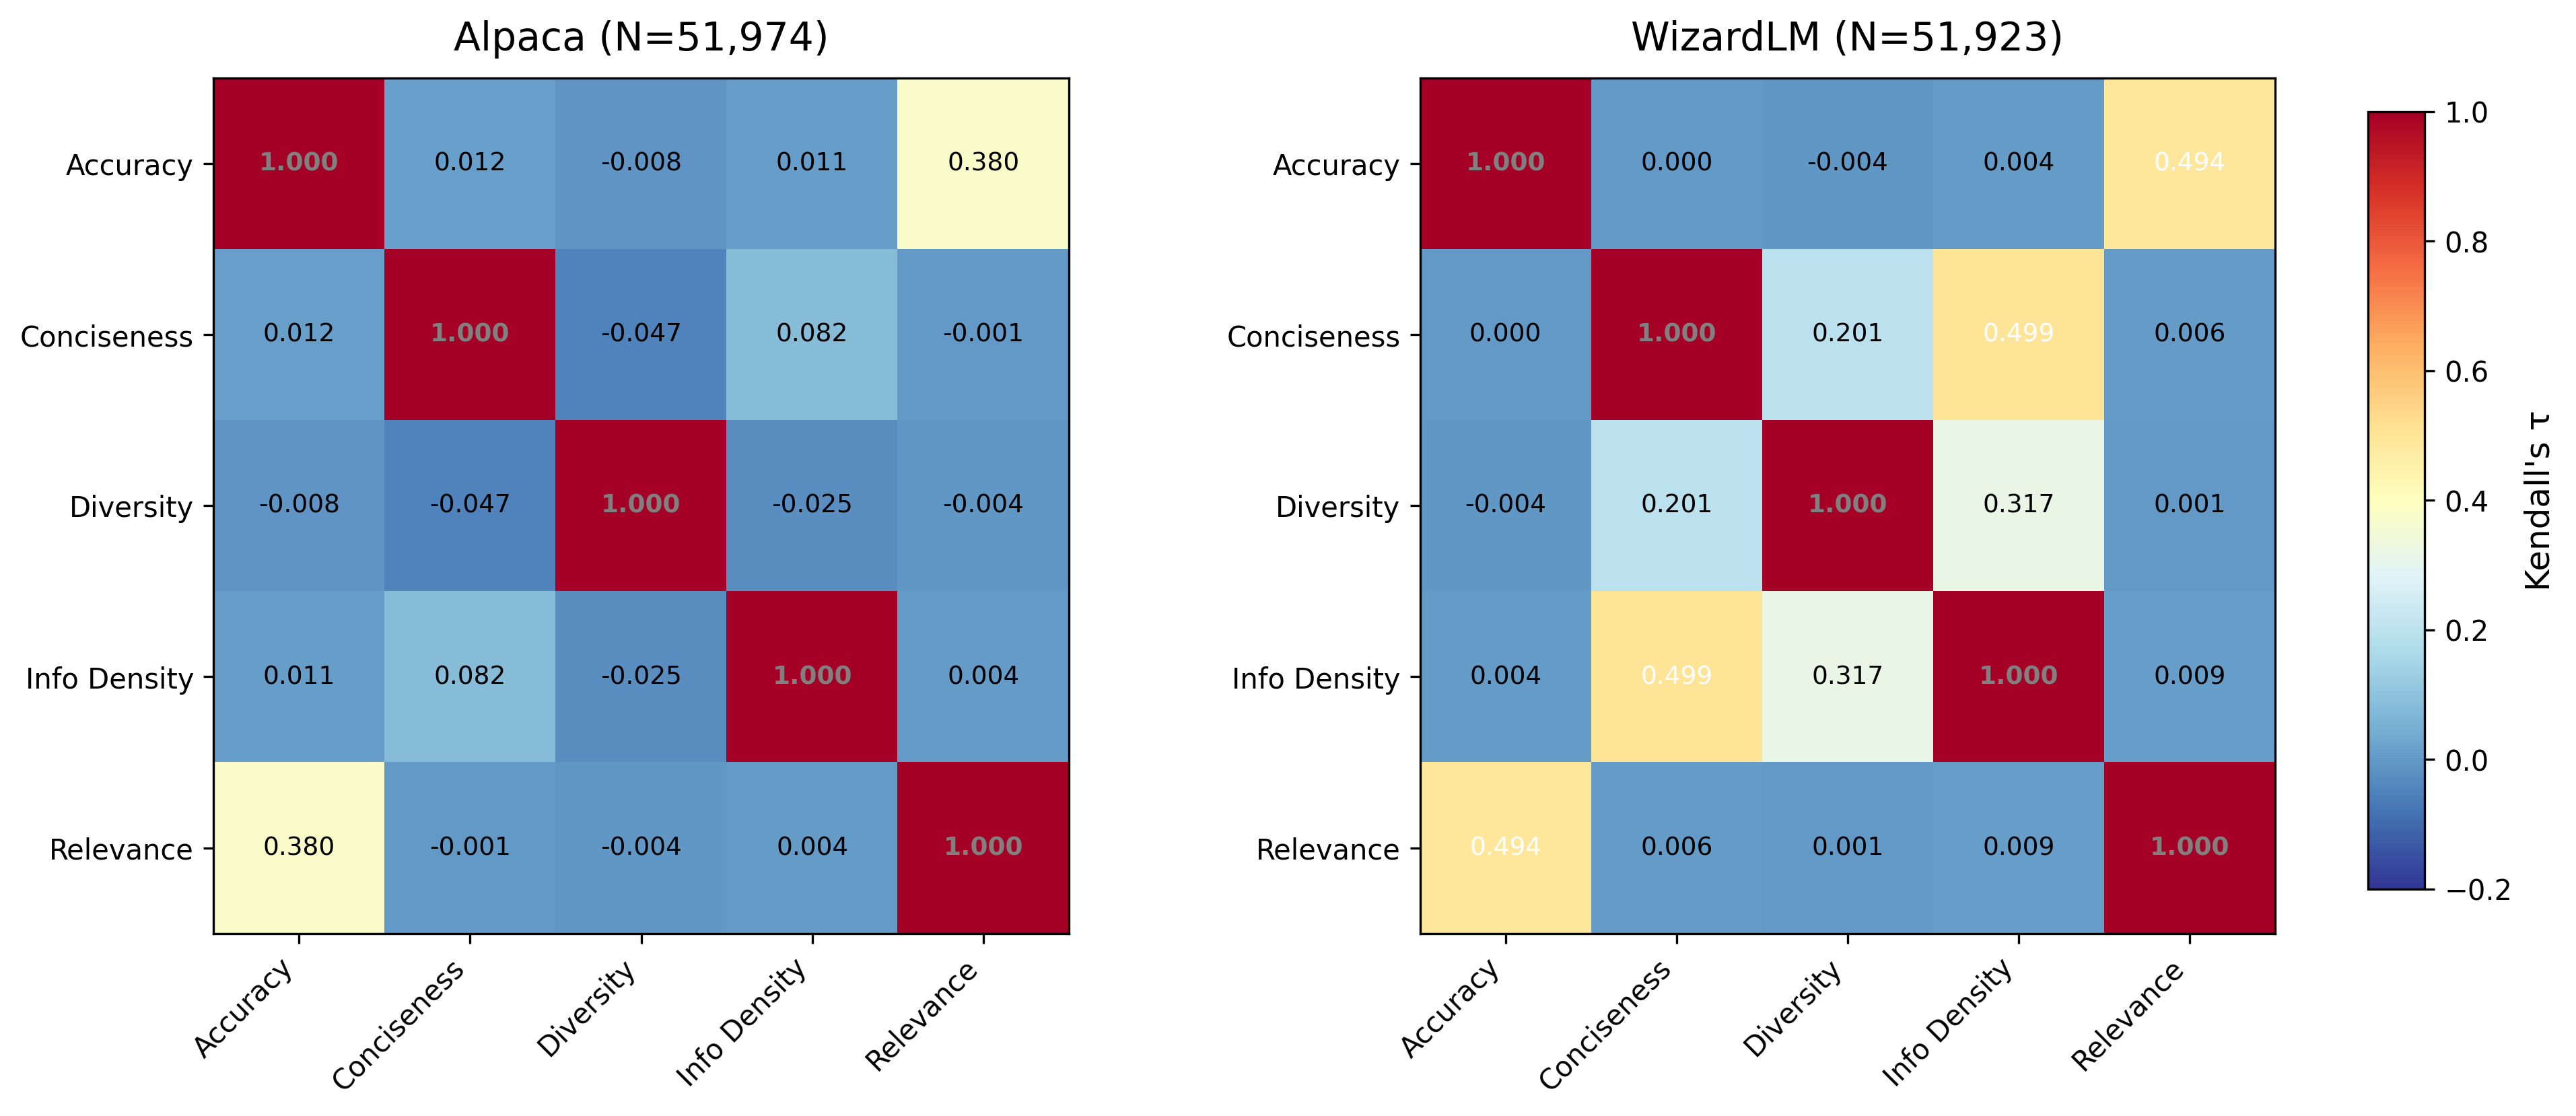
\includegraphics[width=0.82\columnwidth]{paper_tau_comparison.png}
  \caption{Kendall's $\tau$ between quality dimensions for Alpaca (left) and WizardLM (right). In Alpaca, 8 of 10 pairs have $|\tau| < 0.10$; the sole exception is accuracy--relevance ($\tau = 0.380$). WizardLM replicates the cross-group independence but shows moderate within-group correlation among statistical dimensions (conciseness--info\_density $\tau = 0.499$, diversity--info\_density $\tau = 0.317$).}
  \label{fig:tau}
\end{figure}

\begin{figure}[t]
  \centering
  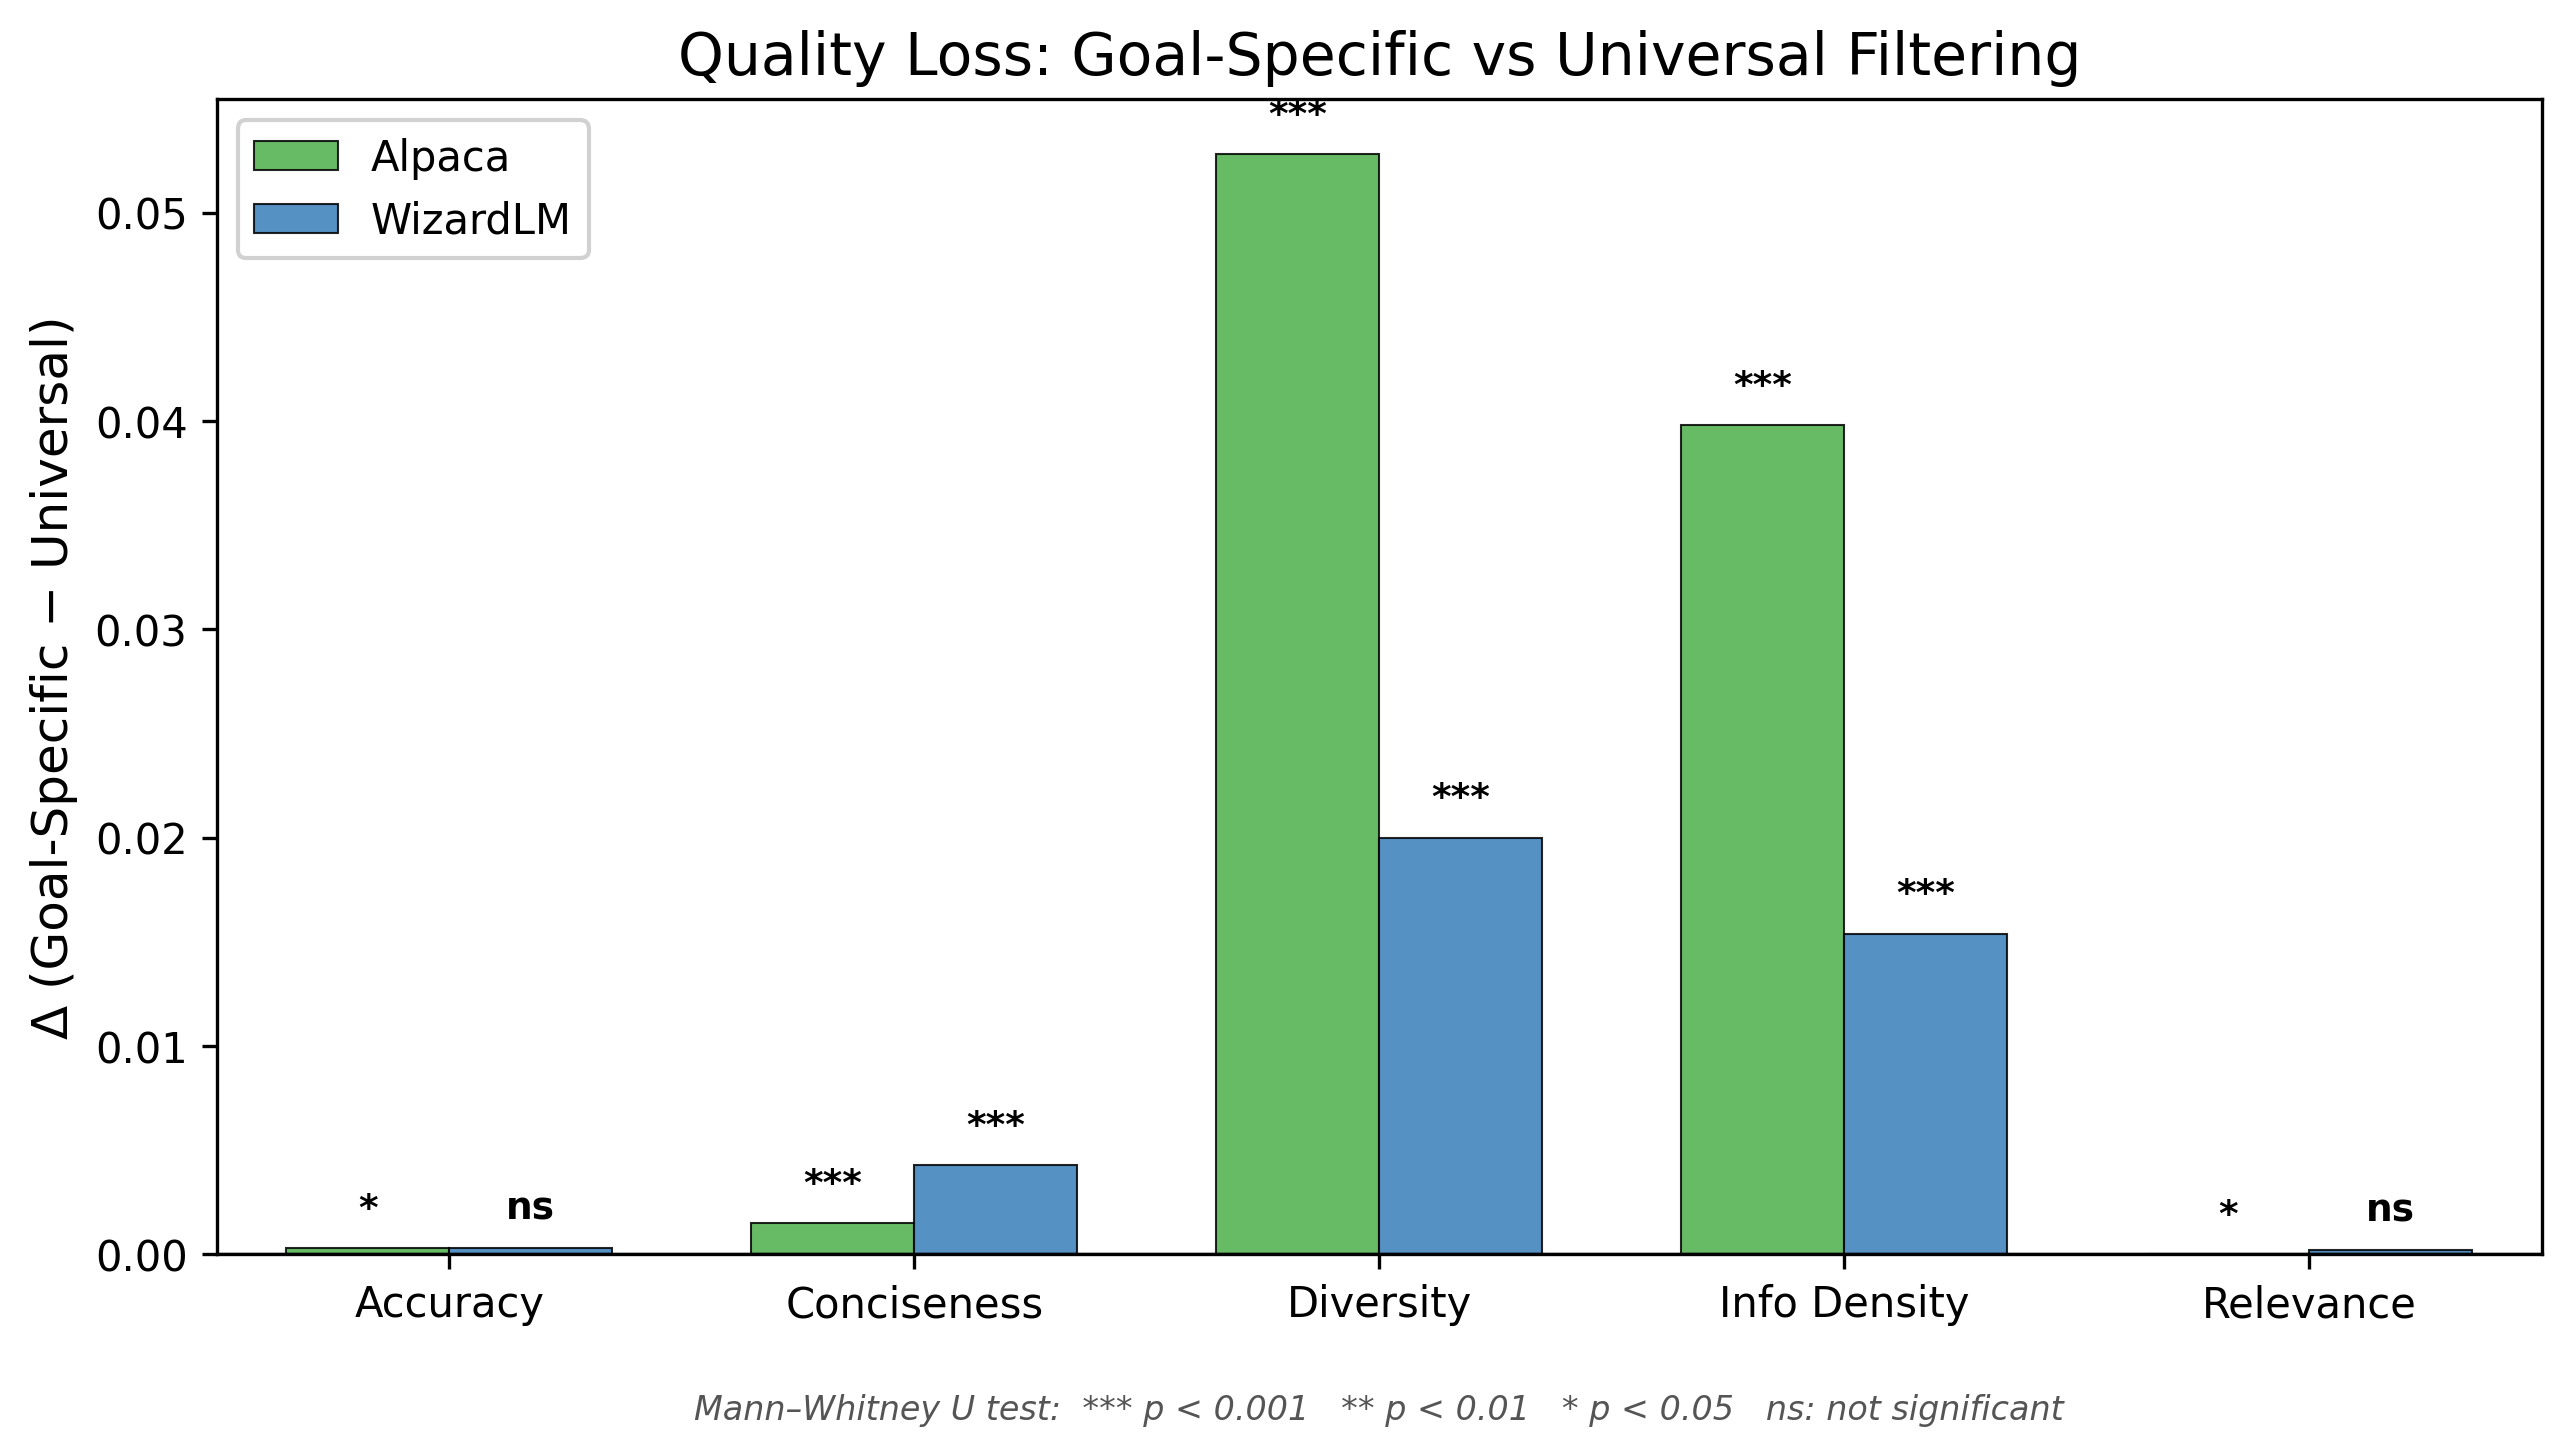
\includegraphics[width=0.82\columnwidth]{paper_quality_loss.png}
  \caption{Score gap ($\Delta$) between goal-specific and universal subsets. Diversity ($\Delta = +0.053$, $r = -0.453$) and information density ($\Delta = +0.040$, $r = -0.349$) suffer the largest losses under universal filtering in Alpaca. WizardLM shows smaller but consistent gaps (diversity $\Delta = +0.020$, info\_density $\Delta = +0.015$, both $p < 0.001$).}
  \label{fig:quality_loss}
\end{figure}

\begin{figure}[t]
  \centering
  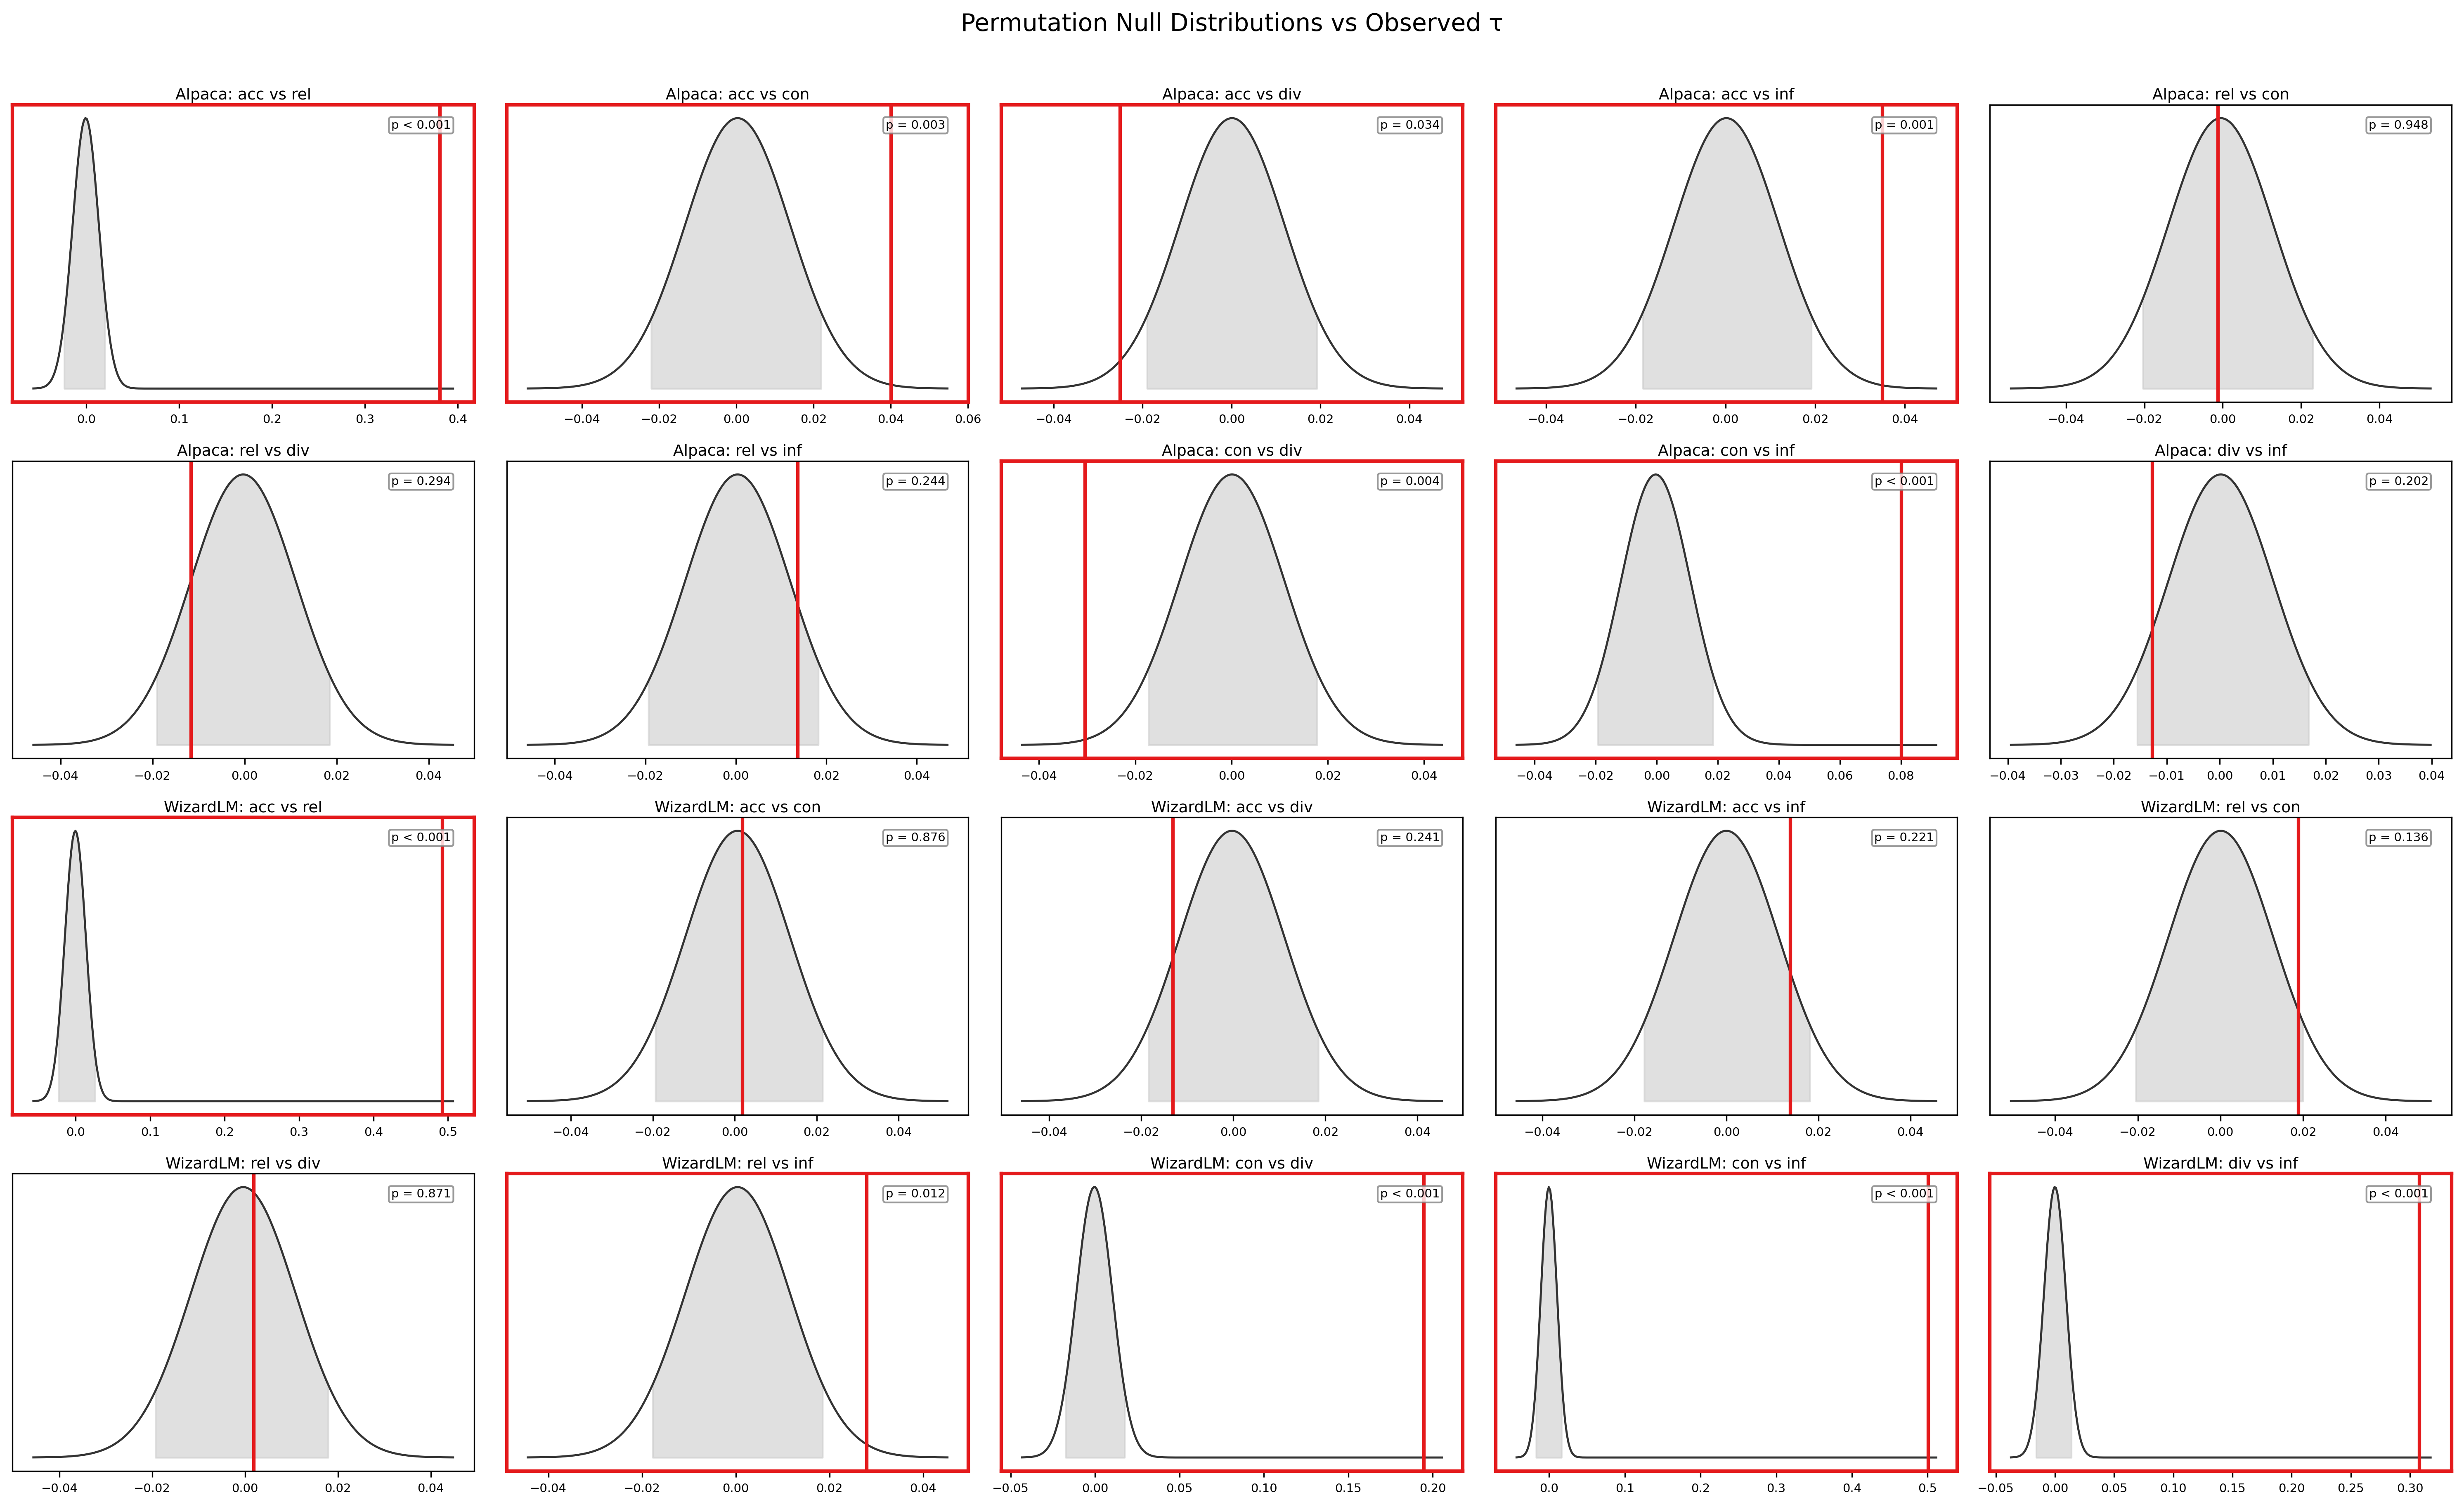
\includegraphics[width=0.82\columnwidth]{paper_permutation_null.png}
  \caption{Permutation null distributions for all 10 dimension pairs (Alpaca, 1{,}000 iterations, $n = 5{,}000$). Red lines mark observed $\tau$. Five pairs (including accuracy--relevance at $\tau = 0.381$, $p = 0.000$; conciseness--info\_density at $\tau = 0.080$, $p = 0.000$) fall outside the null distribution; the remaining five are consistent with independence.}
  \label{fig:permutation}
\end{figure}

\textbf{Near-independence of quality dimensions.}
Figure~\ref{fig:tau} shows that most dimension pairs exhibit near-zero rank correlation.
In Alpaca, the diversity--info\_density Jaccard is $J = 0.154$---fewer than one in six selected examples overlap between these two curated subsets.
The accuracy--relevance pair ($J = 0.991$) reflects shared median-imputation structure rather than genuine overlap (Section~4.7 of the full paper).

\textbf{Quality loss under universal filtering.}
As shown in Figure~\ref{fig:quality_loss}, universal filtering incurs the largest score-distribution gaps on diversity and information density.
We note these deltas are descriptive: goal-specific subsets maximize their target dimension by construction, so the direction of the gap is expected; the magnitude and cross-dataset consistency are the informative quantities.

\textbf{Permutation confirmation.}
Figure~\ref{fig:permutation} confirms that 5 of 10 pairs in Alpaca show statistically detectable rank dependence after Benjamini--Hochberg correction ($p < 0.01$).
The remaining pairs are indistinguishable from the permuted null, consistent with independence.

\textbf{Cross-dataset replication.}
WizardLM replicates the core finding: accuracy--relevance $\tau = 0.494$, all cross-group $|\tau| < 0.01$.
However, statistical dimensions show elevated inter-correlation (conciseness--info\_density $\tau = 0.499$, diversity--info\_density $\tau = 0.317$), suggesting evolutionary generation introduces a shared ``complexity'' factor absent in human-curated data.

\textbf{Downstream validation.}
To test whether score-level divergence translates to trained-model behavior, we finetuned Qwen3.5-0.6B and Qwen3.5-2B~\cite{qwen2025qwen3} on three Alpaca subsets (diversity-optimized, universal composite, random baseline; $N \approx 15{,}593$ per subset; 3 epochs, fixed lr = $2 \times 10^{-5}$, single seed = 42) and evaluated each model on 500 held-out instructions.
The diversity-optimized subset yields the highest Distinct-2 and lowest Self-BLEU at both scales: on Qwen3.5-0.6B, $+5.2$pp Distinct-2 and $-6.9$pp Self-BLEU vs.\ universal; on Qwen3.5-2B, $+5.1$pp and $-6.2$pp.
The ordering diversity-optimized $>$ universal $>$ random $>$ base holds across all diversity metrics and both model sizes, closing the causal gap between score-level divergence and trained-model behavior.

\section{Discussion \& Conclusion}

Our results demonstrate that goal-specific curation strategies produce near-independent subsets for the five quality operationalizations studied.
Composite filtering cannot simultaneously optimize all dimensions: a practitioner optimizing for diversity works with an almost entirely different dataset than one optimizing for information density ($J = 0.154$).

\textbf{Practical implications.}
Researchers should define their curation objective before filtering, dataset publishers should provide multi-dimensional quality metadata, and single-score leaderboards may obscure meaningful per-dimension tradeoffs.
Our downstream validation shifts these recommendations from score-distribution characterization to preliminary evidence of measurable generation differences in trained models.
The statistical protocol (rank-independence screening plus per-dimension Jaccard) is dataset- and modality-agnostic: the same nonparametric tests apply directly to any corpus with $\geq 2$ candidate scoring dimensions, making it straightforward to replicate on multilingual, multimodal, or pretraining data without methodological change.

\textbf{Limitations.}
LLM-as-judge scores for accuracy and relevance are based on 200-sample subsets with median imputation (99.6\% tied), limiting interpretability of $\tau$ for these pairs; our bootstrap reanalysis ($K = 5$, $N = 1{,}000$, no imputation) addresses this only for the subsample.
Our analysis covers two English instruction-tuning datasets; generalization to multilingual, multimodal, or pretraining data is untested.
The downstream validation is small-scale (two model sizes, single training duration, single evaluation set) and should be interpreted as directional evidence rather than definitive proof.

In summary, ``data quality'' in instruction tuning is at least partially multi-dimensional: the five measures studied here cannot be collapsed into a single composite without losing dimension-specific signal, and this score-level divergence produces models with measurably different generation characteristics at Qwen3.5 scales.
Whether the practical gap persists at larger model sizes and extends to task-level performance remains the central open question.

\bibliographystyle{plainnat}
\bibliography{references}

\end{document}
